\documentclass[11pt,pdf,hyperref={unicode}]{beamer}

\beamertemplatenavigationsymbolsempty
\setbeamertemplate{footline}[page number]
% Set it for the internal PhD thesis defence to reduce number of slides
%\setbeamersize{text margin left=0.5em, text margin right=0.5em}

\usepackage[utf8]{inputenc}
\usepackage[english, russian]{babel}
\usepackage{bm}
\usepackage{multirow}
\usepackage{ragged2e}
\usepackage{indentfirst}
\usepackage{multicol}
\usepackage{subfig}
\usepackage{amsmath,amssymb}
\usepackage{enumerate}
\usepackage{mathtools}
\usepackage{comment}
\usepackage[all]{xy}
\usepackage{tikz}
\usetikzlibrary{positioning,arrows}
\tikzstyle{name} = [parameters]
\definecolor{name}{rgb}{0.5,0.5,0.5}

%\usepackage{caption}
%\captionsetup{skip=0pt,belowskip=0pt}

%\newtheorem{theorem}{Theorem}
%\newtheorem{statement}{Statement}
%\newtheorem{definition}{Definition}

% colors
\definecolor{darkgreen}{rgb}{0.0, 0.2, 0.13}
\definecolor{darkcyan}{rgb}{0.0, 0.55, 0.55}
%\AtBeginEnvironment{figure}{\setcounter{subfigure}{0}}
%\captionsetup[subfloat]{labelformat=empty}

%----------------------------------------------------------------------------------------------------------

\title{ Generative or Discriminative?\\
Getting the Best of Both Worlds}
%\author{}
%\institute[]{}
%\date{2024}

%---------------------------------------------------------------------------------------------------------
\begin{document}
%\begin{frame}
%\titlepage
%\end{frame}
\setcounter{page}{2}%remove here for the title
%----------------------------------------------------------------------------------------------------------
%\section{Please do not use sectioning in the presentations}
\begin{frame}{Преобразование прозы в стихотворную форму с помощью методов обработки текста}

\begin{block}{Задача}
    Преобразования прозы в стихотворную форму с заранее заданным размером и рифмовой схемой.
\end{block}
\begin{block}{Метод}
    Использовать архитектуру трансформера LLaMA и применить к ней ограничение вероятностного пространства генерации
\footnote{\textit{Y.~Tian et al.} Zero-shot sonnet generation with discourse-level planning and aesthetics features.~// 2022 Conference of the North
American, 2022.}.
\end{block}
\begin{block}{Решение} 
 Реализация метода ограничения вероятностного пространства генерации к LLaMA и ее дообучение на стихах для преобразования прозы в текст на русском языке.
\end{block}
\end{frame}
%----------------------------------------------------------------------------------------------------------
\begin{frame}{Сравнение вариантов моделей по различным метрикам}

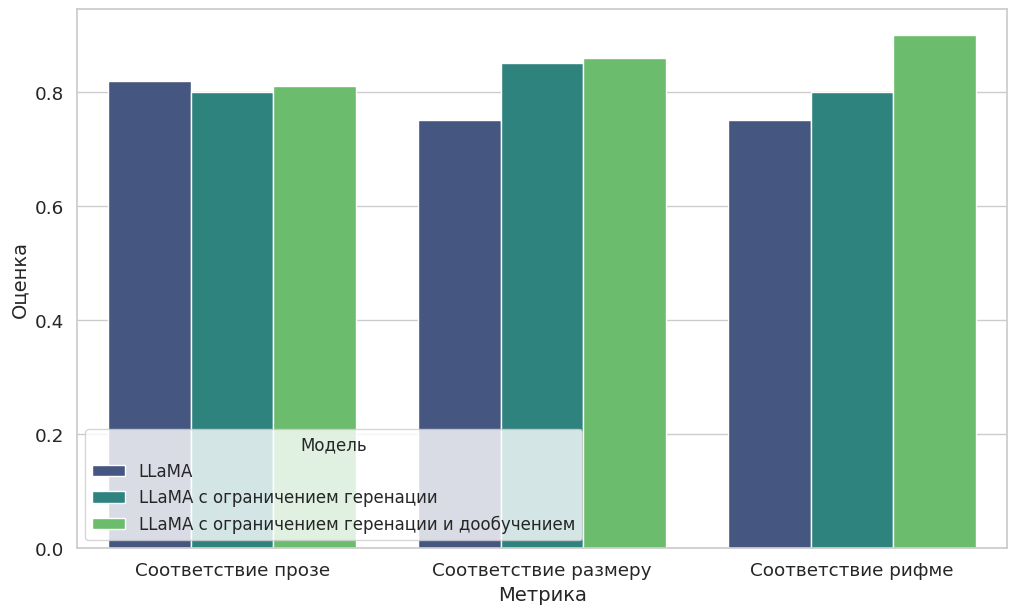
\includegraphics[width=1\textwidth]{image.png}   

Данный график показывает, что за счет небольщого уменьшения в сохранении смысла изначального текста, метод позволяет получать стихи, гораздо лучше соответствующие запросу.
\end{frame}
\end{document}